\documentclass[a4paper, 12pt]{article}
\usepackage{graphicx}
\usepackage{fancyhdr}

\pagestyle{fancy}
\lhead{TDDC78 Lab 5}
\rhead{Hallberg, Svensk}

\begin{document}

\title{TDDC78 Lab 5\\
        Tools }
\author{Christopher Hallberg \\
        Gustav Svensk}
\maketitle

\thispagestyle{empty}

\newpage
\setcounter{page}{1}
\tableofcontents
\newpage

\section{Totalview}
\section{ITAC}
There were some problems using ITAC with full trace where the disc quota on Triolith
was exceeded when using more than a couple of hundred particles. We therefore
ran ITAC twice, one time for the annotated source code with full trace and a
second time with only the MPI tracing functionality. The full trace ran on
four processors with 500 particles each for 30 time steps. The second run without
full tracing used nine processors with 10 000 particles each for 40 time steps.

\subsection{Full Trace}
In the full trace the simulation loop of lab 4 was split into three parts,
collision detection and handling, wall and border crossings and communication. 

\begin{figure}[h]
        \centering
        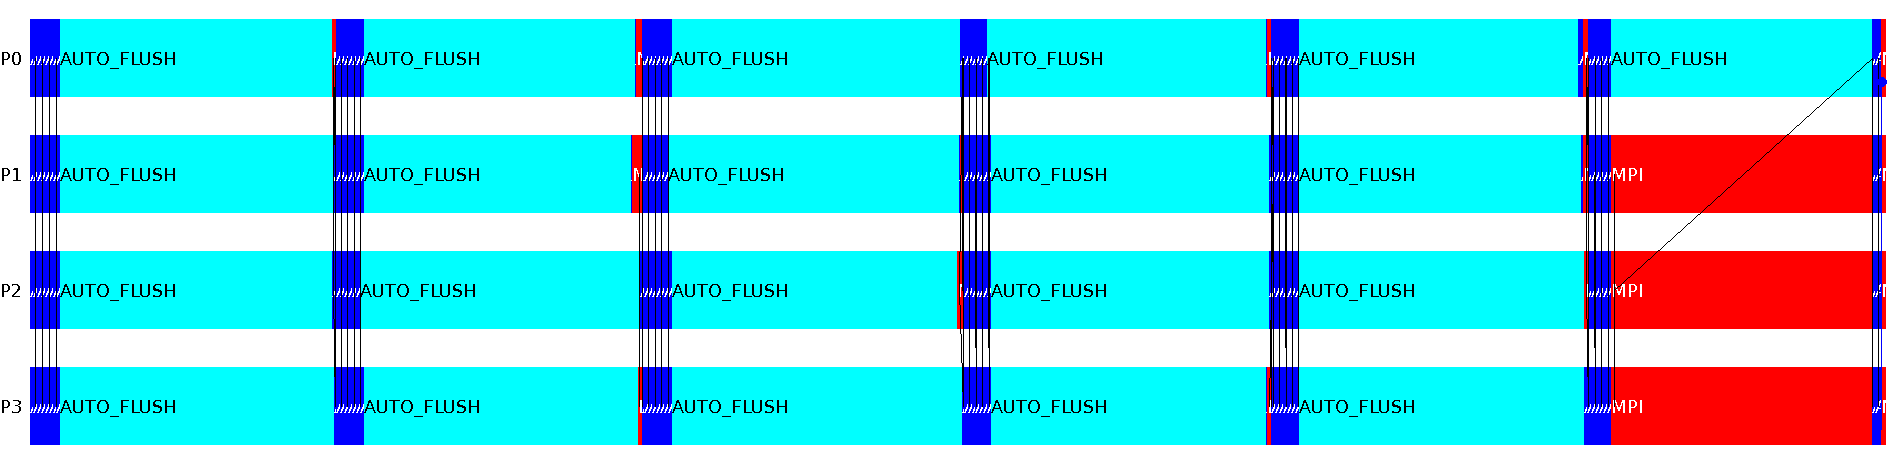
\includegraphics[width=\textwidth]{event_timeline_loop_state.png}
        \caption{Full Trace Timeline}
        \label{fig:ftt}
\end{figure}

\end{document}
